\documentclass[11pt, oneside]{article}   	% use "amsart" instead of "article" for AMSLaTeX format
\usepackage{geometry}                		% See geometry.pdf to learn the layout options. There are lots.
\geometry{letterpaper}                   		% ... or a4paper or a5paper or ... 
\usepackage{graphicx}				% Use pdf, png, jpg, or eps§ with pdflatex; use eps in DVI mode
								% TeX will automatically convert eps --> pdf in pdflatex		
\usepackage{amssymb}
\usepackage{mhchem}


\date{}							% Activate to display a given date or no date
\parindent 0in
\parskip 6pt


 
\begin{document}

\title{\bf Glacier Growth Model}
\maketitle
 
\section*{Learning Goals}
In this lecture we will use conservation of mass to build a simple model of a valley glacier growing in a valley through time.   You will learn about:
\begin{itemize}
\item glacier growth through snow accumulation and loss from melting and sublimation 
\item  glacier movement through internal deformation  and basal sliding 
\item  modeling the time dependent growth of the glacier
\end{itemize}

\section*{Overview}

The first step is to understand how glaciers grow and evolve in shape. Glaciers gain mass by the deposition of snow on the top surface and lose mass through the top surface by a combination of melt and sublimation.  The rate of snowfall and loss is primarily a function of the elevation.  The higher up you are, the more snow.  The lower you are, the more melt and sublimation.  

The Equilibrium Line Altitude (ELA) defines the elevation above which there is more snow than loss and below which there is more loss than snow.  If this were the only process occurring, you would have runaway growth of a glacier above the ELA and never find glaciers below the ELA.  This doesn't occur because glacier ice also moves.  

Glaciers move (or flow) in two main ways:  deformation of the ice and basal sliding of the ice along the base.

In order to build a glacier, we will quantify these rates of ice loss and gain from snow, melt, sublimation, ice deformation and basal sliding.  We will begin with a valley floor elevation profile with no snow, then slowly add snow through time and calculate the evolution of the glacier profile as it grows and moves.

\begin{figure}[htbp]
\begin{center}
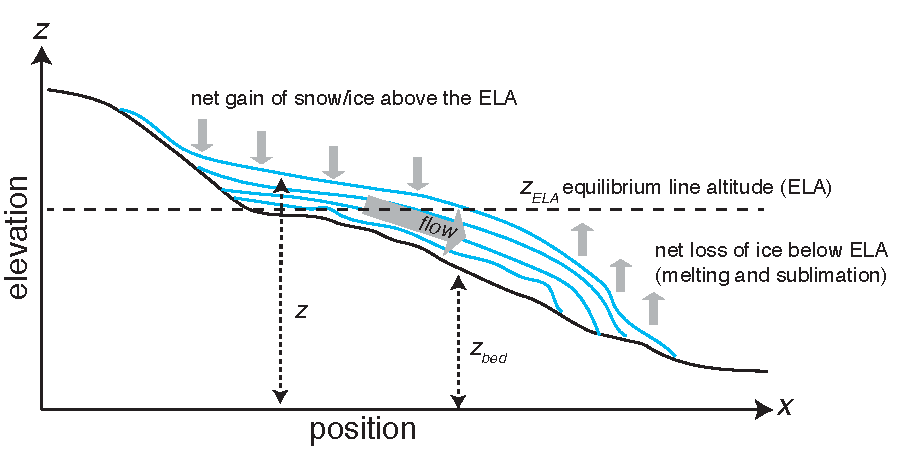
\includegraphics[width=.8\textwidth]{glacier.pdf}
\caption{Valley glacier cross section. Blue lines show the growth of the glacier over time due to mass increase above the equilibrium line altitude (ELA), downhill sliding, internal deformation,  and mass loss below the ELA. }
\label{default}
\end{center}
\end{figure}

%------------------------------------------------------------------------------------------
\section*{Basal Shear Stress} 
%------------------------------------------------------------------------------------------

\begin{figure}[htbp]
\begin{center}
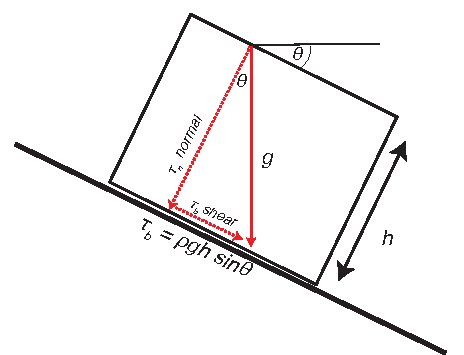
\includegraphics[width=.6\textwidth]{basal.pdf}
\caption{Stress due to the force of gravity $g$ for an ice block with density $\rho$ and thickness $h$.  The downward stress vector can be broken up into a component normal to the slope and one parallel to the slope. The parallel component is known as the basal shear stress $\tau_b$ and depends on the slope angle $\theta$.}
\label{fig:Basal}
\end{center}
\end{figure}

The stress at the bottom of the glacier is the force per unit area on the base of ice.   The force simply from Newton's second law, $F= m a$ after inserting the value of Earth's gravity $g$ for the acceleration, thus $F=mg$. The mass of the ice block is its density times its volume: $m = \rho A h$ where $\rho$ is the ice density, $A$ is the area of the base of the ice block and $h$ is the height.  For a flat lying block of ice, the stress is normal (perpendicular) to the base of the ice block:
\begin{eqnarray}
	\tau_n = F/A =\rho g h.
\end{eqnarray}
What happens when the ice block is tilted, as it is for glaciers flowing down the sides of a mountain or sloping valley? This is shown schematically in Figure \ref{fig:Basal}. In this case the force of gravity can be divided into two vector components: one parallel to and the other perpendicular  to the ice bed.    For a slope angle $\theta$, the normal component $g_\perp = g \cos \theta$ while the parallel component is $g_\parallel = g \sin \theta$.   This parallel component of gravity  creates what is know as basal shear stress $\tau_b$ along the glacier bed. The basal shear stress is simply the parallel force per unit area on the glacier bed:
\begin{eqnarray}
	\tau_b = F_\parallel/A =\rho g_\parallel h = \rho g h \sin \theta.
\end{eqnarray}

Due the basal shear stress, the glacier will slide along its bed. In our model, we will assume the velocity of the base of the glacier as the form
\begin{eqnarray}
	u_s = C_1  \tau_b^2 / (\rho g h) 
\end{eqnarray}
where $C_1$ is the sliding coefficient (m/(Pa yr)), g is gravity (9.81 m/s$^2$). 

In addition to the basal sliding, the shear stress within the glacier allows it to deform plastically.  The deformation velocity when averaged over the thickness of the glacier is:
\begin{eqnarray}
	u_d = 0.4  A h \tau_b^3
\end{eqnarray}
where $ A$ is the Arrhenius constant (Pa$^{-3}$yr$^{-1}$).  

The total lateral velocity of the glacier is then
\begin{eqnarray}
	u = u_d + u_s
\end{eqnarray}


%------------------------------------------------------------------------------------------
\section*{Fluxes} 
%------------------------------------------------------------------------------------------
\begin{figure}[htbp]
\begin{center}
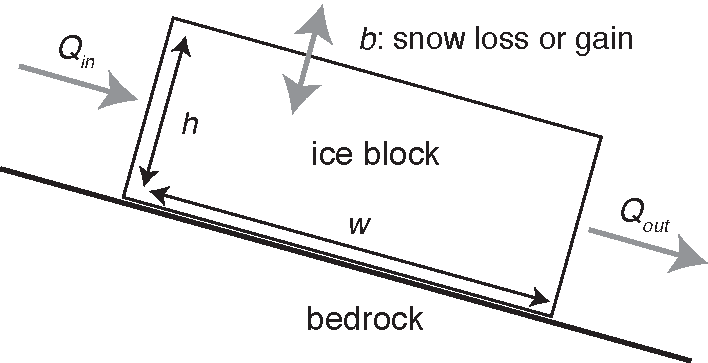
\includegraphics[width=.8\textwidth]{block.pdf}
\caption{Control volume for the glacier growth model.}
\label{default}
\end{center}
\end{figure}
We will assume a model where mass is added to or subtracted to the glacier as a function of position. Above the equilibrium line volume is added due to snowfall, whereas below the ELA volume is loss due to melting and sublimation. We parameterize this as:
\begin{eqnarray}
	b(x) = 0.005 (z- z_{ela}) 
\end{eqnarray}
where here in our 2D problem $b$ will have units of height (m). 

Further, within a given location, we can compute an area flux $Q$ that  lost due to sliding and deformation:
\begin{eqnarray}
	Q = -h ( u_s + u_d)
\end{eqnarray}

Note that $Q$ has units of area per unit time.  Note Also negative sign on the formula for $Q$, since  $Q$ in  means area is being lost, so this means the height is being lowered due to Q. However,  this can be offset by positive b values where snow is accumulating (or it can be further decreased where $b$ is negative.


\begin{figure}[htbp]
\begin{center}
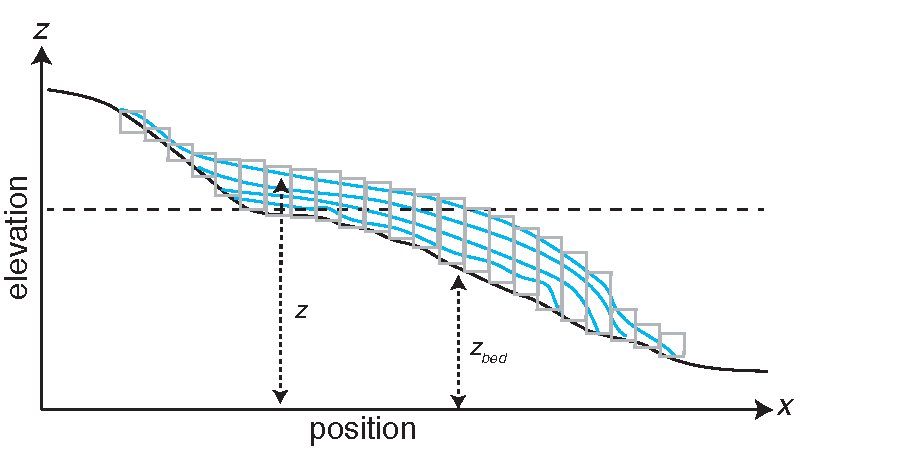
\includegraphics[width=.8\textwidth]{glacier_volumes.pdf}
\caption{Breaking the glacier model up into a series of control volumes (gray boxes) which will be used to conserve mass as a function of time.}
\label{fig:volumes}
\end{center}
\end{figure}


We can break up our glacier model into a series of cells with width $dx$ as shown in Figure \ref{fig:volumes}. At a given instance in time, we can compute $Q$ lost in each cell. Since $Q$ represent the loss of area/unit time , and we have fixed the cell width to be $\Delta x$, the quotient $Q / \Delta x$ then equals the decrease in height of that cell, per unit time due to sliding and deformation. 

Thus we can create a time-stepping simulation where we start with an initial height $h=0$ for every cell. Then we can compute $u_s$, $u_d$ and $Q$ for each cell. We can also compute $b$ for each cell, based on the current elevation of the top of the glacier $z = z_{bed} + h$. The change in height $h$ for the time step is then 
\begin{eqnarray}
	\Delta h = \Delta Q\Delta t/\Delta x + b
\end{eqnarray}


\end{document}  